\documentclass{beamer}
\usetheme{Warsaw}

\usecolortheme[rgb={0.2,0.4,1}]{structure}
\definecolor{grayColor}{rgb}{0.255,0.25,0.275}
\setbeamercolor{section in head/foot}{bg=grayColor,fg=white}

\usepackage[T1]{fontenc}
\usepackage[utf8]{inputenc}
\setbeamertemplate{footline}[frame number]{}
\setbeamertemplate{navigation symbols}{}

\title{Défier l'ordinateur au Sokoban}
\author{Aymeric BEAUCHAMP\\Dimitri CHAGNEUX\\Valentin LEBLOND\\Baptiste MORI}
\date{Avril 2018}

\begin{document} 
\maketitle 

\frame{\tableofcontents}

\section{Objectifs du projet}
\subsection{Description}
\begin{frame} % premier transparent
\frametitle{test}
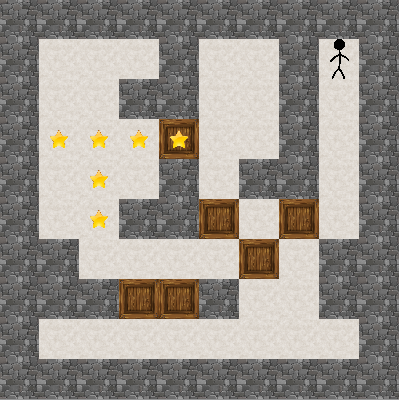
\includegraphics[scale=0.3]{images/sokoban.png}
\end{frame}

\section{Eléments techniques}

\begin{frame}

\end{frame}

\begin{frame}

\end{frame}

\section{Architecture du projet}
\begin{frame}
Architecture du projet
\end{frame}
\section{Expérimentations et usages}
\begin{frame}
Expérimentations et usages
\end{frame}
\section{Conclusion}
\begin{frame}
Conclusion
\end{frame}
\end{document}
